% Created by tikzDevice version 0.12.6 on 2026-08-12 14:25:22
% !TEX encoding = UTF-8 Unicode
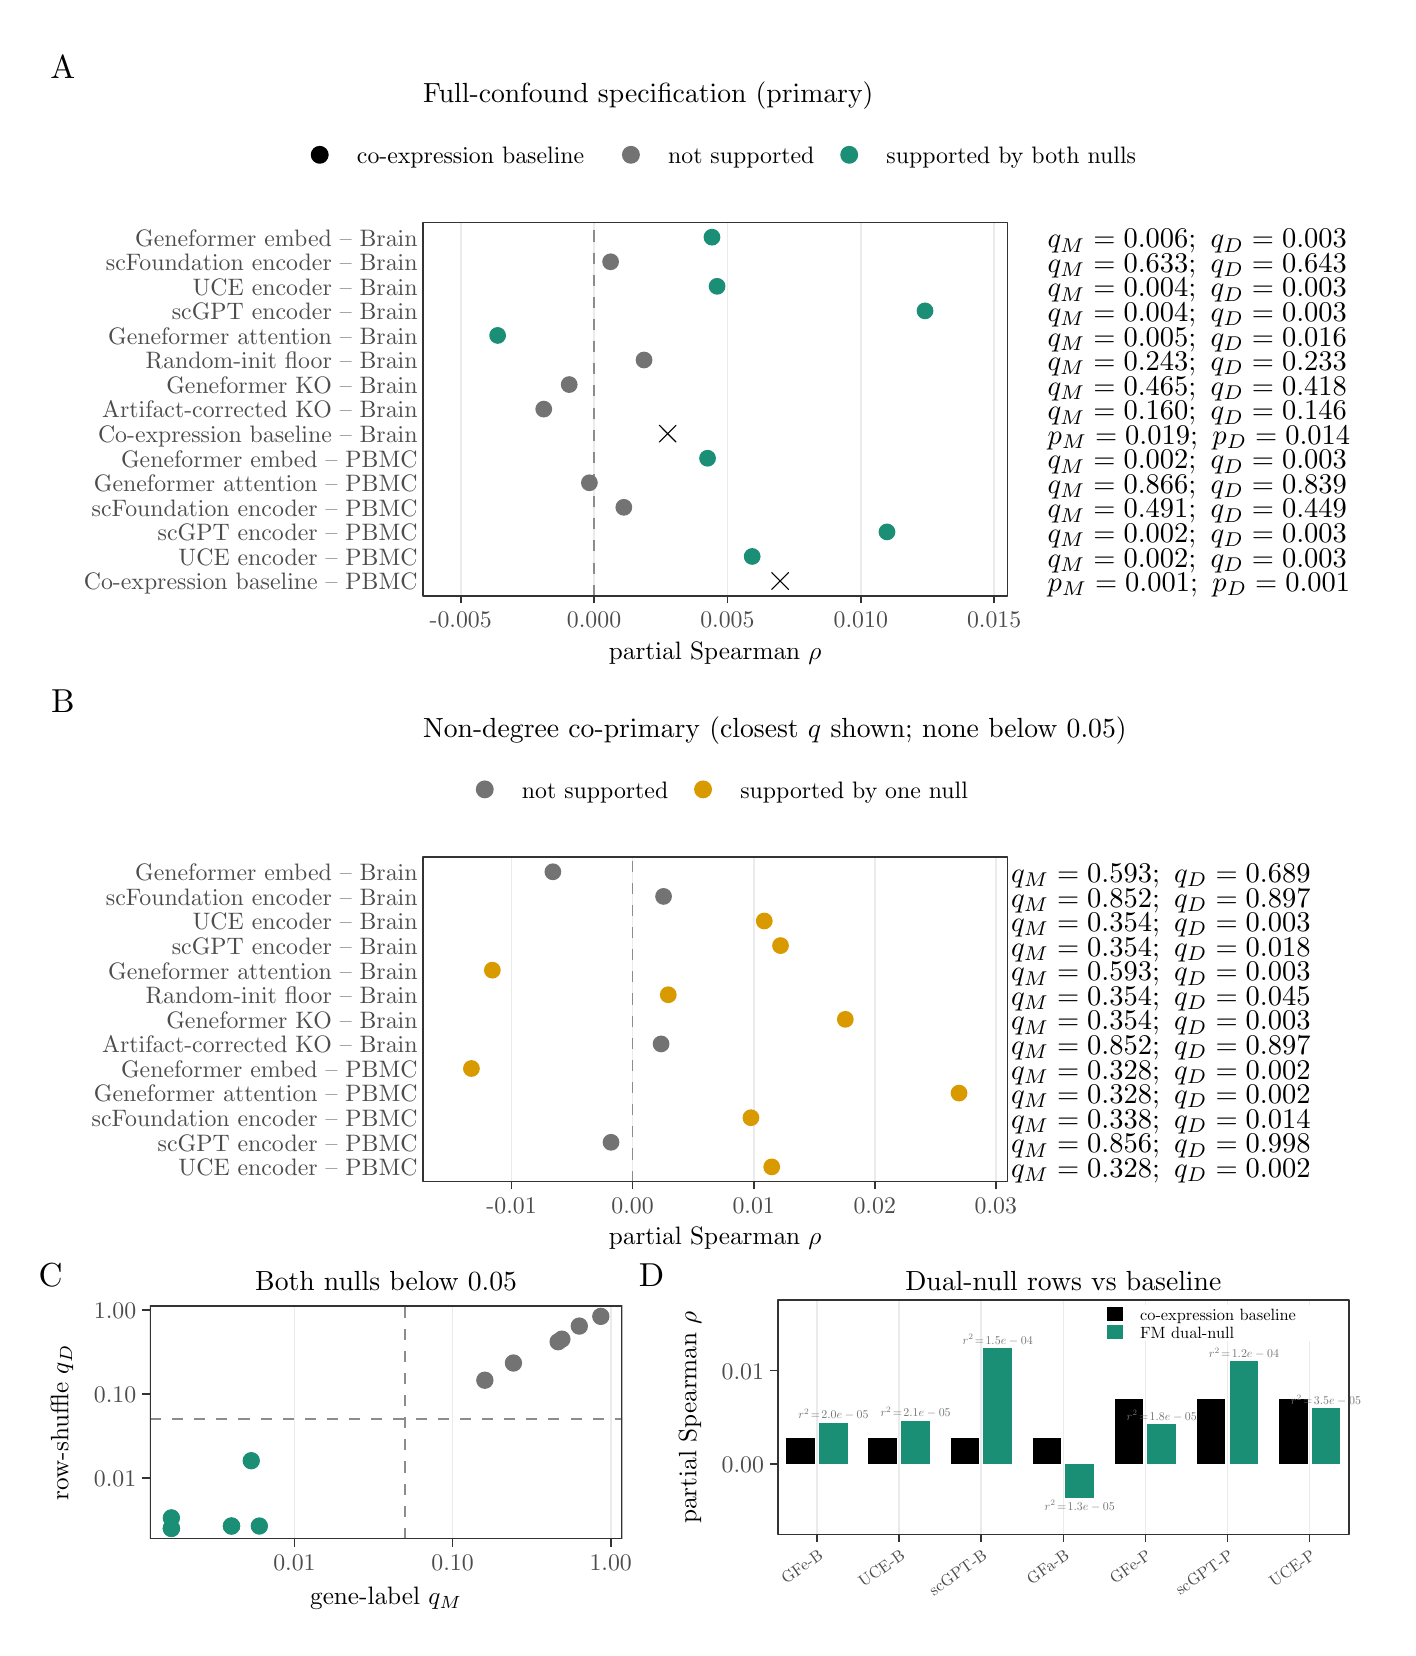
\begin{tikzpicture}[x=1pt,y=1pt]
\definecolor{fillColor}{RGB}{255,255,255}
\path[use as bounding box,fill=fillColor,fill opacity=0.00] (0,0) rectangle (491.44,578.16);
\begin{scope}
\path[clip] (  0.00,  0.00) rectangle (491.44,578.16);
\definecolor{drawColor}{RGB}{255,255,255}
\definecolor{fillColor}{RGB}{255,255,255}

\path[draw=drawColor,line width= 0.6pt,line join=round,line cap=round,fill=fillColor] ( -0.00,  0.00) rectangle (491.44,578.16);
\end{scope}
\begin{scope}
\path[clip] (  4.00,  3.00) rectangle (485.44,133.15);
\definecolor{drawColor}{RGB}{255,255,255}
\definecolor{fillColor}{RGB}{255,255,255}

\path[draw=drawColor,line width= 0.6pt,line join=round,line cap=round,fill=fillColor] (  4.00,  3.00) rectangle (485.44,133.15);
\end{scope}
\begin{scope}
\path[clip] (  4.00,344.86) rectangle (485.44,574.16);
\definecolor{drawColor}{RGB}{255,255,255}
\definecolor{fillColor}{RGB}{255,255,255}

\path[draw=drawColor,line width= 0.6pt,line join=round,line cap=round,fill=fillColor] (  4.00,344.86) rectangle (485.44,574.16);
\end{scope}
\begin{scope}
\path[clip] (  4.00,133.15) rectangle (485.44,344.86);
\definecolor{drawColor}{RGB}{255,255,255}
\definecolor{fillColor}{RGB}{255,255,255}

\path[draw=drawColor,line width= 0.6pt,line join=round,line cap=round,fill=fillColor] (  4.00,133.15) rectangle (485.44,344.86);
\end{scope}
\begin{scope}
\path[clip] (  0.00,  0.00) rectangle (491.44,578.16);
\definecolor{fillColor}{RGB}{255,255,255}

\path[fill=fillColor] (142.87,372.88) rectangle (354.02,507.76);
\definecolor{drawColor}{gray}{0.92}

\path[draw=drawColor,line width= 0.6pt,line join=round] (156.48,372.88) --
	(156.48,507.76);

\path[draw=drawColor,line width= 0.6pt,line join=round] (204.67,372.88) --
	(204.67,507.76);

\path[draw=drawColor,line width= 0.6pt,line join=round] (252.86,372.88) --
	(252.86,507.76);

\path[draw=drawColor,line width= 0.6pt,line join=round] (301.05,372.88) --
	(301.05,507.76);

\path[draw=drawColor,line width= 0.6pt,line join=round] (349.24,372.88) --
	(349.24,507.76);
\definecolor{drawColor}{gray}{0.55}

\path[draw=drawColor,line width= 0.6pt,dash pattern=on 4pt off 4pt ,line join=round] (204.67,372.88) -- (204.67,507.76);
\definecolor{fillColor}{RGB}{27,143,117}

\path[fill=fillColor] (247.27,502.44) circle (  3.03);
\definecolor{fillColor}{gray}{0.45}

\path[fill=fillColor] (210.64,493.56) circle (  3.03);
\definecolor{fillColor}{RGB}{27,143,117}

\path[fill=fillColor] (249.12,484.69) circle (  3.03);

\path[fill=fillColor] (324.25,475.82) circle (  3.03);

\path[fill=fillColor] (169.82,466.94) circle (  3.03);
\definecolor{fillColor}{gray}{0.45}

\path[fill=fillColor] (222.72,458.07) circle (  3.03);

\path[fill=fillColor] (195.68,449.19) circle (  3.03);

\path[fill=fillColor] (186.48,440.32) circle (  3.03);
\definecolor{drawColor}{RGB}{0,0,0}

\path[draw=drawColor,line width= 0.4pt,line join=round,line cap=round] (228.24,428.41) -- (234.30,434.48);

\path[draw=drawColor,line width= 0.4pt,line join=round,line cap=round] (228.24,434.48) -- (234.30,428.41);
\definecolor{fillColor}{RGB}{27,143,117}

\path[fill=fillColor] (245.67,422.57) circle (  3.03);
\definecolor{fillColor}{gray}{0.45}

\path[fill=fillColor] (202.98,413.70) circle (  3.03);

\path[fill=fillColor] (215.42,404.83) circle (  3.03);
\definecolor{fillColor}{RGB}{27,143,117}

\path[fill=fillColor] (310.51,395.95) circle (  3.03);

\path[fill=fillColor] (261.80,387.08) circle (  3.03);

\path[draw=drawColor,line width= 0.4pt,line join=round,line cap=round] (268.86,375.17) -- (274.92,381.24);

\path[draw=drawColor,line width= 0.4pt,line join=round,line cap=round] (268.86,381.24) -- (274.92,375.17);

\node[text=drawColor,anchor=base west,inner sep=0pt, outer sep=0pt, scale=  1.03] at (368.52,498.61) {$q_M=0.006;\ q_D=0.003$};

\node[text=drawColor,anchor=base west,inner sep=0pt, outer sep=0pt, scale=  1.03] at (368.52,489.73) {$q_M=0.633;\ q_D=0.643$};

\node[text=drawColor,anchor=base west,inner sep=0pt, outer sep=0pt, scale=  1.03] at (368.52,480.86) {$q_M=0.004;\ q_D=0.003$};

\node[text=drawColor,anchor=base west,inner sep=0pt, outer sep=0pt, scale=  1.03] at (368.52,471.98) {$q_M=0.004;\ q_D=0.003$};

\node[text=drawColor,anchor=base west,inner sep=0pt, outer sep=0pt, scale=  1.03] at (368.52,463.11) {$q_M=0.005;\ q_D=0.016$};

\node[text=drawColor,anchor=base west,inner sep=0pt, outer sep=0pt, scale=  1.03] at (368.52,454.24) {$q_M=0.243;\ q_D=0.233$};

\node[text=drawColor,anchor=base west,inner sep=0pt, outer sep=0pt, scale=  1.03] at (368.52,445.36) {$q_M=0.465;\ q_D=0.418$};

\node[text=drawColor,anchor=base west,inner sep=0pt, outer sep=0pt, scale=  1.03] at (368.52,436.49) {$q_M=0.160;\ q_D=0.146$};

\node[text=drawColor,anchor=base west,inner sep=0pt, outer sep=0pt, scale=  1.03] at (368.52,427.62) {$p_M=0.019;\ p_D=0.014$};

\node[text=drawColor,anchor=base west,inner sep=0pt, outer sep=0pt, scale=  1.03] at (368.52,418.74) {$q_M=0.002;\ q_D=0.003$};

\node[text=drawColor,anchor=base west,inner sep=0pt, outer sep=0pt, scale=  1.03] at (368.52,409.87) {$q_M=0.866;\ q_D=0.839$};

\node[text=drawColor,anchor=base west,inner sep=0pt, outer sep=0pt, scale=  1.03] at (368.52,401.00) {$q_M=0.491;\ q_D=0.449$};

\node[text=drawColor,anchor=base west,inner sep=0pt, outer sep=0pt, scale=  1.03] at (368.52,392.12) {$q_M=0.002;\ q_D=0.003$};

\node[text=drawColor,anchor=base west,inner sep=0pt, outer sep=0pt, scale=  1.03] at (368.52,383.25) {$q_M=0.002;\ q_D=0.003$};

\node[text=drawColor,anchor=base west,inner sep=0pt, outer sep=0pt, scale=  1.03] at (368.52,374.38) {$p_M=0.001;\ p_D=0.001$};
\definecolor{drawColor}{gray}{0.20}

\path[draw=drawColor,line width= 0.6pt,line join=round,line cap=round] (142.87,372.88) rectangle (354.02,507.76);
\end{scope}
\begin{scope}
\path[clip] (  0.00,  0.00) rectangle (491.44,578.16);
\definecolor{drawColor}{gray}{0.30}

\node[text=drawColor,anchor=base east,inner sep=0pt, outer sep=0pt, scale=  0.86] at (140.87,375.01) {Co-expression baseline -- PBMC};

\node[text=drawColor,anchor=base east,inner sep=0pt, outer sep=0pt, scale=  0.86] at (140.87,383.88) {UCE encoder -- PBMC};

\node[text=drawColor,anchor=base east,inner sep=0pt, outer sep=0pt, scale=  0.86] at (140.87,392.76) {scGPT encoder -- PBMC};

\node[text=drawColor,anchor=base east,inner sep=0pt, outer sep=0pt, scale=  0.86] at (140.87,401.63) {scFoundation encoder -- PBMC};

\node[text=drawColor,anchor=base east,inner sep=0pt, outer sep=0pt, scale=  0.86] at (140.87,410.50) {Geneformer attention -- PBMC};

\node[text=drawColor,anchor=base east,inner sep=0pt, outer sep=0pt, scale=  0.86] at (140.87,419.38) {Geneformer embed -- PBMC};

\node[text=drawColor,anchor=base east,inner sep=0pt, outer sep=0pt, scale=  0.86] at (140.87,428.25) {Co-expression baseline -- Brain};

\node[text=drawColor,anchor=base east,inner sep=0pt, outer sep=0pt, scale=  0.86] at (140.87,437.13) {Artifact-corrected KO -- Brain};

\node[text=drawColor,anchor=base east,inner sep=0pt, outer sep=0pt, scale=  0.86] at (140.87,446.00) {Geneformer KO -- Brain};

\node[text=drawColor,anchor=base east,inner sep=0pt, outer sep=0pt, scale=  0.86] at (140.87,454.87) {Random-init floor -- Brain};

\node[text=drawColor,anchor=base east,inner sep=0pt, outer sep=0pt, scale=  0.86] at (140.87,463.75) {Geneformer attention -- Brain};

\node[text=drawColor,anchor=base east,inner sep=0pt, outer sep=0pt, scale=  0.86] at (140.87,472.62) {scGPT encoder -- Brain};

\node[text=drawColor,anchor=base east,inner sep=0pt, outer sep=0pt, scale=  0.86] at (140.87,481.49) {UCE encoder -- Brain};

\node[text=drawColor,anchor=base east,inner sep=0pt, outer sep=0pt, scale=  0.86] at (140.87,490.37) {scFoundation encoder -- Brain};

\node[text=drawColor,anchor=base east,inner sep=0pt, outer sep=0pt, scale=  0.86] at (140.87,499.24) {Geneformer embed -- Brain};
\end{scope}
\begin{scope}
\path[clip] (  0.00,  0.00) rectangle (491.44,578.16);
\definecolor{drawColor}{gray}{0.20}

\path[draw=drawColor,line width= 0.6pt,line join=round] (156.48,370.13) --
	(156.48,372.88);

\path[draw=drawColor,line width= 0.6pt,line join=round] (204.67,370.13) --
	(204.67,372.88);

\path[draw=drawColor,line width= 0.6pt,line join=round] (252.86,370.13) --
	(252.86,372.88);

\path[draw=drawColor,line width= 0.6pt,line join=round] (301.05,370.13) --
	(301.05,372.88);

\path[draw=drawColor,line width= 0.6pt,line join=round] (349.24,370.13) --
	(349.24,372.88);
\end{scope}
\begin{scope}
\path[clip] (  0.00,  0.00) rectangle (491.44,578.16);
\definecolor{drawColor}{gray}{0.30}

\node[text=drawColor,anchor=base,inner sep=0pt, outer sep=0pt, scale=  0.86] at (156.48,361.54) {-0.005};

\node[text=drawColor,anchor=base,inner sep=0pt, outer sep=0pt, scale=  0.86] at (204.67,361.54) {0.000};

\node[text=drawColor,anchor=base,inner sep=0pt, outer sep=0pt, scale=  0.86] at (252.86,361.54) {0.005};

\node[text=drawColor,anchor=base,inner sep=0pt, outer sep=0pt, scale=  0.86] at (301.05,361.54) {0.010};

\node[text=drawColor,anchor=base,inner sep=0pt, outer sep=0pt, scale=  0.86] at (349.24,361.54) {0.015};
\end{scope}
\begin{scope}
\path[clip] (  0.00,  0.00) rectangle (491.44,578.16);
\definecolor{drawColor}{RGB}{0,0,0}

\node[text=drawColor,anchor=base,inner sep=0pt, outer sep=0pt, scale=  0.91] at (248.45,350.01) {partial Spearman $\rho$};
\end{scope}
\begin{scope}
\path[clip] (  0.00,  0.00) rectangle (491.44,578.16);
\definecolor{fillColor}{RGB}{255,255,255}

\path[fill=fillColor] ( 92.08,518.76) rectangle (404.81,545.66);
\end{scope}
\begin{scope}
\path[clip] (  0.00,  0.00) rectangle (491.44,578.16);
\definecolor{fillColor}{RGB}{255,255,255}

\path[fill=fillColor] ( 97.58,524.26) rectangle (113.48,540.16);
\definecolor{drawColor}{RGB}{0,0,0}
\definecolor{fillColor}{RGB}{0,0,0}

\path[draw=drawColor,line width= 0.4pt,line join=round,line cap=round,fill=fillColor] (105.53,532.21) circle (  3.03);
\end{scope}
\begin{scope}
\path[clip] (  0.00,  0.00) rectangle (491.44,578.16);
\definecolor{fillColor}{RGB}{255,255,255}

\path[fill=fillColor] (210.03,524.26) rectangle (225.93,540.16);
\definecolor{drawColor}{gray}{0.45}
\definecolor{fillColor}{gray}{0.45}

\path[draw=drawColor,line width= 0.4pt,line join=round,line cap=round,fill=fillColor] (217.98,532.21) circle (  3.03);
\end{scope}
\begin{scope}
\path[clip] (  0.00,  0.00) rectangle (491.44,578.16);
\definecolor{fillColor}{RGB}{255,255,255}

\path[fill=fillColor] (288.91,524.26) rectangle (304.81,540.16);
\definecolor{drawColor}{RGB}{27,143,117}
\definecolor{fillColor}{RGB}{27,143,117}

\path[draw=drawColor,line width= 0.4pt,line join=round,line cap=round,fill=fillColor] (296.86,532.21) circle (  3.03);
\end{scope}
\begin{scope}
\path[clip] (  0.00,  0.00) rectangle (491.44,578.16);
\definecolor{drawColor}{RGB}{0,0,0}

\node[text=drawColor,anchor=base west,inner sep=0pt, outer sep=0pt, scale=  0.86] at (118.98,529.01) {co-expression baseline};
\end{scope}
\begin{scope}
\path[clip] (  0.00,  0.00) rectangle (491.44,578.16);
\definecolor{drawColor}{RGB}{0,0,0}

\node[text=drawColor,anchor=base west,inner sep=0pt, outer sep=0pt, scale=  0.86] at (231.43,529.01) {not supported};
\end{scope}
\begin{scope}
\path[clip] (  0.00,  0.00) rectangle (491.44,578.16);
\definecolor{drawColor}{RGB}{0,0,0}

\node[text=drawColor,anchor=base west,inner sep=0pt, outer sep=0pt, scale=  0.86] at (310.31,529.01) {supported by both nulls};
\end{scope}
\begin{scope}
\path[clip] (  0.00,  0.00) rectangle (491.44,578.16);
\definecolor{drawColor}{RGB}{0,0,0}

\node[text=drawColor,anchor=base west,inner sep=0pt, outer sep=0pt, scale=  1.00] at (142.87,551.03) {Full-confound specification (primary)};
\end{scope}
\begin{scope}
\path[clip] (  0.00,  0.00) rectangle (491.44,578.16);
\definecolor{drawColor}{RGB}{0,0,0}

\node[text=drawColor,anchor=base,inner sep=0pt, outer sep=0pt, scale=  1.20] at ( 12.74,559.86) {A};
\end{scope}
\begin{scope}
\path[clip] (  0.00,  0.00) rectangle (491.44,578.16);
\definecolor{fillColor}{RGB}{255,255,255}

\path[fill=fillColor] (142.87,161.17) rectangle (354.02,278.46);
\definecolor{drawColor}{gray}{0.92}

\path[draw=drawColor,line width= 0.6pt,line join=round] (174.86,161.17) --
	(174.86,278.46);

\path[draw=drawColor,line width= 0.6pt,line join=round] (218.60,161.17) --
	(218.60,278.46);

\path[draw=drawColor,line width= 0.6pt,line join=round] (262.34,161.17) --
	(262.34,278.46);

\path[draw=drawColor,line width= 0.6pt,line join=round] (306.09,161.17) --
	(306.09,278.46);

\path[draw=drawColor,line width= 0.6pt,line join=round] (349.83,161.17) --
	(349.83,278.46);
\definecolor{drawColor}{gray}{0.55}

\path[draw=drawColor,line width= 0.6pt,dash pattern=on 4pt off 4pt ,line join=round] (218.60,161.17) -- (218.60,278.46);
\definecolor{fillColor}{gray}{0.45}

\path[fill=fillColor] (189.78,273.13) circle (  3.03);

\path[fill=fillColor] (229.78,264.24) circle (  3.03);
\definecolor{fillColor}{RGB}{217,154,0}

\path[fill=fillColor] (266.17,255.36) circle (  3.03);

\path[fill=fillColor] (272.04,246.47) circle (  3.03);

\path[fill=fillColor] (167.91,237.59) circle (  3.03);

\path[fill=fillColor] (231.48,228.70) circle (  3.03);

\path[fill=fillColor] (295.45,219.82) circle (  3.03);
\definecolor{fillColor}{gray}{0.45}

\path[fill=fillColor] (228.88,210.93) circle (  3.03);
\definecolor{fillColor}{RGB}{217,154,0}

\path[fill=fillColor] (160.35,202.05) circle (  3.03);

\path[fill=fillColor] (336.55,193.16) circle (  3.03);

\path[fill=fillColor] (261.35,184.27) circle (  3.03);
\definecolor{fillColor}{gray}{0.45}

\path[fill=fillColor] (210.79,175.39) circle (  3.03);
\definecolor{fillColor}{RGB}{217,154,0}

\path[fill=fillColor] (268.86,166.50) circle (  3.03);
\definecolor{drawColor}{RGB}{0,0,0}

\node[text=drawColor,anchor=base west,inner sep=0pt, outer sep=0pt, scale=  1.03] at (355.36,269.30) {$q_M=0.593;\ q_D=0.689$};

\node[text=drawColor,anchor=base west,inner sep=0pt, outer sep=0pt, scale=  1.03] at (355.36,260.41) {$q_M=0.852;\ q_D=0.897$};

\node[text=drawColor,anchor=base west,inner sep=0pt, outer sep=0pt, scale=  1.03] at (355.36,251.53) {$q_M=0.354;\ q_D=0.003$};

\node[text=drawColor,anchor=base west,inner sep=0pt, outer sep=0pt, scale=  1.03] at (355.36,242.64) {$q_M=0.354;\ q_D=0.018$};

\node[text=drawColor,anchor=base west,inner sep=0pt, outer sep=0pt, scale=  1.03] at (355.36,233.76) {$q_M=0.593;\ q_D=0.003$};

\node[text=drawColor,anchor=base west,inner sep=0pt, outer sep=0pt, scale=  1.03] at (355.36,224.87) {$q_M=0.354;\ q_D=0.045$};

\node[text=drawColor,anchor=base west,inner sep=0pt, outer sep=0pt, scale=  1.03] at (355.36,215.98) {$q_M=0.354;\ q_D=0.003$};

\node[text=drawColor,anchor=base west,inner sep=0pt, outer sep=0pt, scale=  1.03] at (355.36,207.10) {$q_M=0.852;\ q_D=0.897$};

\node[text=drawColor,anchor=base west,inner sep=0pt, outer sep=0pt, scale=  1.03] at (355.36,198.21) {$q_M=0.328;\ q_D=0.002$};

\node[text=drawColor,anchor=base west,inner sep=0pt, outer sep=0pt, scale=  1.03] at (355.36,189.33) {$q_M=0.328;\ q_D=0.002$};

\node[text=drawColor,anchor=base west,inner sep=0pt, outer sep=0pt, scale=  1.03] at (355.36,180.44) {$q_M=0.338;\ q_D=0.014$};

\node[text=drawColor,anchor=base west,inner sep=0pt, outer sep=0pt, scale=  1.03] at (355.36,171.56) {$q_M=0.856;\ q_D=0.998$};

\node[text=drawColor,anchor=base west,inner sep=0pt, outer sep=0pt, scale=  1.03] at (355.36,162.67) {$q_M=0.328;\ q_D=0.002$};
\definecolor{drawColor}{gray}{0.20}

\path[draw=drawColor,line width= 0.6pt,line join=round,line cap=round] (142.87,161.17) rectangle (354.02,278.46);
\end{scope}
\begin{scope}
\path[clip] (  0.00,  0.00) rectangle (491.44,578.16);
\definecolor{drawColor}{gray}{0.30}

\node[text=drawColor,anchor=base east,inner sep=0pt, outer sep=0pt, scale=  0.86] at (140.87,163.31) {UCE encoder -- PBMC};

\node[text=drawColor,anchor=base east,inner sep=0pt, outer sep=0pt, scale=  0.86] at (140.87,172.19) {scGPT encoder -- PBMC};

\node[text=drawColor,anchor=base east,inner sep=0pt, outer sep=0pt, scale=  0.86] at (140.87,181.08) {scFoundation encoder -- PBMC};

\node[text=drawColor,anchor=base east,inner sep=0pt, outer sep=0pt, scale=  0.86] at (140.87,189.96) {Geneformer attention -- PBMC};

\node[text=drawColor,anchor=base east,inner sep=0pt, outer sep=0pt, scale=  0.86] at (140.87,198.85) {Geneformer embed -- PBMC};

\node[text=drawColor,anchor=base east,inner sep=0pt, outer sep=0pt, scale=  0.86] at (140.87,207.73) {Artifact-corrected KO -- Brain};

\node[text=drawColor,anchor=base east,inner sep=0pt, outer sep=0pt, scale=  0.86] at (140.87,216.62) {Geneformer KO -- Brain};

\node[text=drawColor,anchor=base east,inner sep=0pt, outer sep=0pt, scale=  0.86] at (140.87,225.50) {Random-init floor -- Brain};

\node[text=drawColor,anchor=base east,inner sep=0pt, outer sep=0pt, scale=  0.86] at (140.87,234.39) {Geneformer attention -- Brain};

\node[text=drawColor,anchor=base east,inner sep=0pt, outer sep=0pt, scale=  0.86] at (140.87,243.28) {scGPT encoder -- Brain};

\node[text=drawColor,anchor=base east,inner sep=0pt, outer sep=0pt, scale=  0.86] at (140.87,252.16) {UCE encoder -- Brain};

\node[text=drawColor,anchor=base east,inner sep=0pt, outer sep=0pt, scale=  0.86] at (140.87,261.05) {scFoundation encoder -- Brain};

\node[text=drawColor,anchor=base east,inner sep=0pt, outer sep=0pt, scale=  0.86] at (140.87,269.93) {Geneformer embed -- Brain};
\end{scope}
\begin{scope}
\path[clip] (  0.00,  0.00) rectangle (491.44,578.16);
\definecolor{drawColor}{gray}{0.20}

\path[draw=drawColor,line width= 0.6pt,line join=round] (174.86,158.42) --
	(174.86,161.17);

\path[draw=drawColor,line width= 0.6pt,line join=round] (218.60,158.42) --
	(218.60,161.17);

\path[draw=drawColor,line width= 0.6pt,line join=round] (262.34,158.42) --
	(262.34,161.17);

\path[draw=drawColor,line width= 0.6pt,line join=round] (306.09,158.42) --
	(306.09,161.17);

\path[draw=drawColor,line width= 0.6pt,line join=round] (349.83,158.42) --
	(349.83,161.17);
\end{scope}
\begin{scope}
\path[clip] (  0.00,  0.00) rectangle (491.44,578.16);
\definecolor{drawColor}{gray}{0.30}

\node[text=drawColor,anchor=base,inner sep=0pt, outer sep=0pt, scale=  0.86] at (174.86,149.83) {-0.01};

\node[text=drawColor,anchor=base,inner sep=0pt, outer sep=0pt, scale=  0.86] at (218.60,149.83) {0.00};

\node[text=drawColor,anchor=base,inner sep=0pt, outer sep=0pt, scale=  0.86] at (262.34,149.83) {0.01};

\node[text=drawColor,anchor=base,inner sep=0pt, outer sep=0pt, scale=  0.86] at (306.09,149.83) {0.02};

\node[text=drawColor,anchor=base,inner sep=0pt, outer sep=0pt, scale=  0.86] at (349.83,149.83) {0.03};
\end{scope}
\begin{scope}
\path[clip] (  0.00,  0.00) rectangle (491.44,578.16);
\definecolor{drawColor}{RGB}{0,0,0}

\node[text=drawColor,anchor=base,inner sep=0pt, outer sep=0pt, scale=  0.91] at (248.45,138.30) {partial Spearman $\rho$};
\end{scope}
\begin{scope}
\path[clip] (  0.00,  0.00) rectangle (491.44,578.16);
\definecolor{fillColor}{RGB}{255,255,255}

\path[fill=fillColor] (151.72,289.46) rectangle (345.17,316.36);
\end{scope}
\begin{scope}
\path[clip] (  0.00,  0.00) rectangle (491.44,578.16);
\definecolor{fillColor}{RGB}{255,255,255}

\path[fill=fillColor] (157.22,294.96) rectangle (173.12,310.86);
\definecolor{drawColor}{gray}{0.45}
\definecolor{fillColor}{gray}{0.45}

\path[draw=drawColor,line width= 0.4pt,line join=round,line cap=round,fill=fillColor] (165.17,302.91) circle (  3.03);
\end{scope}
\begin{scope}
\path[clip] (  0.00,  0.00) rectangle (491.44,578.16);
\definecolor{fillColor}{RGB}{255,255,255}

\path[fill=fillColor] (236.10,294.96) rectangle (252.00,310.86);
\definecolor{drawColor}{RGB}{217,154,0}
\definecolor{fillColor}{RGB}{217,154,0}

\path[draw=drawColor,line width= 0.4pt,line join=round,line cap=round,fill=fillColor] (244.05,302.91) circle (  3.03);
\end{scope}
\begin{scope}
\path[clip] (  0.00,  0.00) rectangle (491.44,578.16);
\definecolor{drawColor}{RGB}{0,0,0}

\node[text=drawColor,anchor=base west,inner sep=0pt, outer sep=0pt, scale=  0.86] at (178.62,299.71) {not supported};
\end{scope}
\begin{scope}
\path[clip] (  0.00,  0.00) rectangle (491.44,578.16);
\definecolor{drawColor}{RGB}{0,0,0}

\node[text=drawColor,anchor=base west,inner sep=0pt, outer sep=0pt, scale=  0.86] at (257.50,299.71) {supported by one null};
\end{scope}
\begin{scope}
\path[clip] (  0.00,  0.00) rectangle (491.44,578.16);
\definecolor{drawColor}{RGB}{0,0,0}

\node[text=drawColor,anchor=base west,inner sep=0pt, outer sep=0pt, scale=  1.00] at (142.87,321.73) {Non-degree co-primary (closest $q$ shown; none below 0.05)};
\end{scope}
\begin{scope}
\path[clip] (  0.00,  0.00) rectangle (491.44,578.16);
\definecolor{drawColor}{RGB}{0,0,0}

\node[text=drawColor,anchor=base,inner sep=0pt, outer sep=0pt, scale=  1.20] at ( 12.74,330.55) {B};
\end{scope}
\begin{scope}
\path[clip] (  4.00,  3.00) rectangle (220.86,133.15);
\definecolor{drawColor}{RGB}{255,255,255}
\definecolor{fillColor}{RGB}{255,255,255}

\path[draw=drawColor,line width= 0.6pt,line join=round,line cap=round,fill=fillColor] (  4.00,  3.00) rectangle (220.86,133.15);
\end{scope}
\begin{scope}
\path[clip] ( 44.17, 32.05) rectangle (214.86,116.32);
\definecolor{fillColor}{RGB}{255,255,255}

\path[fill=fillColor] ( 44.17, 32.05) rectangle (214.86,116.32);
\definecolor{drawColor}{gray}{0.92}

\path[draw=drawColor,line width= 0.6pt,line join=round] ( 96.39, 32.05) --
	( 96.39,116.32);

\path[draw=drawColor,line width= 0.6pt,line join=round] (153.53, 32.05) --
	(153.53,116.32);

\path[draw=drawColor,line width= 0.6pt,line join=round] (210.67, 32.05) --
	(210.67,116.32);
\definecolor{drawColor}{gray}{0.55}

\path[draw=drawColor,line width= 0.6pt,dash pattern=on 4pt off 4pt ,line join=round] (136.33, 32.05) -- (136.33,116.32);

\path[draw=drawColor,line width= 0.6pt,dash pattern=on 4pt off 4pt ,line join=round] ( 44.17, 75.34) -- (214.86, 75.34);
\definecolor{drawColor}{RGB}{27,143,117}
\definecolor{fillColor}{RGB}{27,143,117}

\path[draw=drawColor,line width= 0.4pt,line join=round,line cap=round,fill=fillColor] ( 83.71, 36.73) circle (  2.93);
\definecolor{drawColor}{gray}{0.45}
\definecolor{fillColor}{gray}{0.45}

\path[draw=drawColor,line width= 0.4pt,line join=round,line cap=round,fill=fillColor] (199.33,108.98) circle (  2.93);
\definecolor{drawColor}{RGB}{27,143,117}
\definecolor{fillColor}{RGB}{27,143,117}

\path[draw=drawColor,line width= 0.4pt,line join=round,line cap=round,fill=fillColor] ( 73.65, 36.73) circle (  2.93);

\path[draw=drawColor,line width= 0.4pt,line join=round,line cap=round,fill=fillColor] ( 73.65, 36.73) circle (  2.93);

\path[draw=drawColor,line width= 0.4pt,line join=round,line cap=round,fill=fillColor] ( 80.79, 60.33) circle (  2.93);
\definecolor{drawColor}{gray}{0.45}
\definecolor{fillColor}{gray}{0.45}

\path[draw=drawColor,line width= 0.4pt,line join=round,line cap=round,fill=fillColor] (175.53, 95.63) circle (  2.93);

\path[draw=drawColor,line width= 0.4pt,line join=round,line cap=round,fill=fillColor] (191.68,103.32) circle (  2.93);

\path[draw=drawColor,line width= 0.4pt,line join=round,line cap=round,fill=fillColor] (165.20, 89.42) circle (  2.93);
\definecolor{drawColor}{RGB}{27,143,117}
\definecolor{fillColor}{RGB}{27,143,117}

\path[draw=drawColor,line width= 0.4pt,line join=round,line cap=round,fill=fillColor] ( 51.93, 39.67) circle (  2.93);
\definecolor{drawColor}{gray}{0.45}
\definecolor{fillColor}{gray}{0.45}

\path[draw=drawColor,line width= 0.4pt,line join=round,line cap=round,fill=fillColor] (207.10,112.49) circle (  2.93);

\path[draw=drawColor,line width= 0.4pt,line join=round,line cap=round,fill=fillColor] (193.03,104.25) circle (  2.93);
\definecolor{drawColor}{RGB}{27,143,117}
\definecolor{fillColor}{RGB}{27,143,117}

\path[draw=drawColor,line width= 0.4pt,line join=round,line cap=round,fill=fillColor] ( 51.93, 35.88) circle (  2.93);

\path[draw=drawColor,line width= 0.4pt,line join=round,line cap=round,fill=fillColor] ( 51.93, 35.88) circle (  2.93);
\definecolor{drawColor}{gray}{0.20}

\path[draw=drawColor,line width= 0.6pt,line join=round,line cap=round] ( 44.17, 32.05) rectangle (214.86,116.32);
\end{scope}
\begin{scope}
\path[clip] (  0.00,  0.00) rectangle (491.44,578.16);
\definecolor{drawColor}{gray}{0.30}

\node[text=drawColor,anchor=base east,inner sep=0pt, outer sep=0pt, scale=  0.86] at ( 39.22, 50.95) {0.01};

\node[text=drawColor,anchor=base east,inner sep=0pt, outer sep=0pt, scale=  0.86] at ( 39.22, 81.27) {0.10};

\node[text=drawColor,anchor=base east,inner sep=0pt, outer sep=0pt, scale=  0.86] at ( 39.22,111.60) {1.00};
\end{scope}
\begin{scope}
\path[clip] (  0.00,  0.00) rectangle (491.44,578.16);
\definecolor{drawColor}{gray}{0.20}

\path[draw=drawColor,line width= 0.6pt,line join=round] ( 41.42, 54.14) --
	( 44.17, 54.14);

\path[draw=drawColor,line width= 0.6pt,line join=round] ( 41.42, 84.47) --
	( 44.17, 84.47);

\path[draw=drawColor,line width= 0.6pt,line join=round] ( 41.42,114.80) --
	( 44.17,114.80);
\end{scope}
\begin{scope}
\path[clip] (  0.00,  0.00) rectangle (491.44,578.16);
\definecolor{drawColor}{gray}{0.20}

\path[draw=drawColor,line width= 0.6pt,line join=round] ( 96.39, 29.30) --
	( 96.39, 32.05);

\path[draw=drawColor,line width= 0.6pt,line join=round] (153.53, 29.30) --
	(153.53, 32.05);

\path[draw=drawColor,line width= 0.6pt,line join=round] (210.67, 29.30) --
	(210.67, 32.05);
\end{scope}
\begin{scope}
\path[clip] (  0.00,  0.00) rectangle (491.44,578.16);
\definecolor{drawColor}{gray}{0.30}

\node[text=drawColor,anchor=base,inner sep=0pt, outer sep=0pt, scale=  0.86] at ( 96.39, 20.71) {0.01};

\node[text=drawColor,anchor=base,inner sep=0pt, outer sep=0pt, scale=  0.86] at (153.53, 20.71) {0.10};

\node[text=drawColor,anchor=base,inner sep=0pt, outer sep=0pt, scale=  0.86] at (210.67, 20.71) {1.00};
\end{scope}
\begin{scope}
\path[clip] (  0.00,  0.00) rectangle (491.44,578.16);
\definecolor{drawColor}{RGB}{0,0,0}

\node[text=drawColor,anchor=base,inner sep=0pt, outer sep=0pt, scale=  0.91] at (129.52,  8.21) {gene-label $q_M$};
\end{scope}
\begin{scope}
\path[clip] (  0.00,  0.00) rectangle (491.44,578.16);
\definecolor{drawColor}{RGB}{0,0,0}

\node[text=drawColor,rotate= 90.00,anchor=base,inner sep=0pt, outer sep=0pt, scale=  0.91] at ( 14.73, 74.18) {row-shuffle $q_D$};
\end{scope}
\begin{scope}
\path[clip] (  0.00,  0.00) rectangle (491.44,578.16);
\definecolor{drawColor}{RGB}{0,0,0}

\node[text=drawColor,anchor=base,inner sep=0pt, outer sep=0pt, scale=  1.00] at (129.52,121.75) {Both nulls below 0.05};
\end{scope}
\begin{scope}
\path[clip] (  0.00,  0.00) rectangle (491.44,578.16);
\definecolor{drawColor}{RGB}{0,0,0}

\node[text=drawColor,anchor=base west,inner sep=0pt, outer sep=0pt, scale=  1.20] at (  4.00,123.38) {C};
\end{scope}
\begin{scope}
\path[clip] (220.86,  3.00) rectangle (485.44,133.15);
\definecolor{drawColor}{RGB}{255,255,255}
\definecolor{fillColor}{RGB}{255,255,255}

\path[draw=drawColor,line width= 0.6pt,line join=round,line cap=round,fill=fillColor] (220.86,  3.00) rectangle (485.44,133.15);
\end{scope}
\begin{scope}
\path[clip] (  0.00,  0.00) rectangle (491.44,578.16);
\definecolor{fillColor}{RGB}{255,255,255}

\path[fill=fillColor] (271.03, 33.71) rectangle (477.44,118.32);
\definecolor{drawColor}{gray}{0.92}

\path[draw=drawColor,line width= 0.6pt,line join=round] (285.27, 33.71) --
	(285.27,118.32);

\path[draw=drawColor,line width= 0.6pt,line join=round] (314.92, 33.71) --
	(314.92,118.32);

\path[draw=drawColor,line width= 0.6pt,line join=round] (344.58, 33.71) --
	(344.58,118.32);

\path[draw=drawColor,line width= 0.6pt,line join=round] (374.23, 33.71) --
	(374.23,118.32);

\path[draw=drawColor,line width= 0.6pt,line join=round] (403.89, 33.71) --
	(403.89,118.32);

\path[draw=drawColor,line width= 0.6pt,line join=round] (433.55, 33.71) --
	(433.55,118.32);

\path[draw=drawColor,line width= 0.6pt,line join=round] (463.20, 33.71) --
	(463.20,118.32);
\definecolor{fillColor}{RGB}{27,143,117}

\path[fill=fillColor] (286.01, 59.20) rectangle (296.39, 74.12);
\definecolor{fillColor}{RGB}{0,0,0}

\path[fill=fillColor] (274.15, 59.20) rectangle (284.53, 68.52);
\definecolor{fillColor}{RGB}{27,143,117}

\path[fill=fillColor] (315.67, 59.20) rectangle (326.04, 74.77);
\definecolor{fillColor}{RGB}{0,0,0}

\path[fill=fillColor] (303.80, 59.20) rectangle (314.18, 68.52);
\definecolor{fillColor}{RGB}{27,143,117}

\path[fill=fillColor] (345.32, 59.20) rectangle (355.70,101.07);
\definecolor{fillColor}{RGB}{0,0,0}

\path[fill=fillColor] (333.46, 59.20) rectangle (343.84, 68.52);
\definecolor{fillColor}{RGB}{27,143,117}

\path[fill=fillColor] (374.98, 47.00) rectangle (385.36, 59.20);
\definecolor{fillColor}{RGB}{0,0,0}

\path[fill=fillColor] (363.11, 59.20) rectangle (373.49, 68.52);
\definecolor{fillColor}{RGB}{27,143,117}

\path[fill=fillColor] (404.63, 59.20) rectangle (415.01, 73.56);
\definecolor{fillColor}{RGB}{0,0,0}

\path[fill=fillColor] (392.77, 59.20) rectangle (403.15, 82.74);
\definecolor{fillColor}{RGB}{27,143,117}

\path[fill=fillColor] (434.29, 59.20) rectangle (444.67, 96.26);
\definecolor{fillColor}{RGB}{0,0,0}

\path[fill=fillColor] (422.43, 59.20) rectangle (432.80, 82.74);
\definecolor{fillColor}{RGB}{27,143,117}

\path[fill=fillColor] (463.94, 59.20) rectangle (474.32, 79.21);
\definecolor{fillColor}{RGB}{0,0,0}

\path[fill=fillColor] (452.08, 59.20) rectangle (462.46, 82.74);
\definecolor{drawColor}{gray}{0.45}

\node[text=drawColor,anchor=base,inner sep=0pt, outer sep=0pt, scale=  0.43] at (291.20, 75.54) {$r^{2}\!=\!2.0e-05$};

\node[text=drawColor,anchor=base,inner sep=0pt, outer sep=0pt, scale=  0.43] at (320.85, 76.19) {$r^{2}\!=\!2.1e-05$};

\node[text=drawColor,anchor=base,inner sep=0pt, outer sep=0pt, scale=  0.43] at (350.51,102.49) {$r^{2}\!=\!1.5e-04$};

\node[text=drawColor,anchor=base,inner sep=0pt, outer sep=0pt, scale=  0.43] at (380.17, 42.42) {$r^{2}\!=\!1.3e-05$};

\node[text=drawColor,anchor=base,inner sep=0pt, outer sep=0pt, scale=  0.43] at (409.82, 74.98) {$r^{2}\!=\!1.8e-05$};

\node[text=drawColor,anchor=base,inner sep=0pt, outer sep=0pt, scale=  0.43] at (439.48, 97.68) {$r^{2}\!=\!1.2e-04$};

\node[text=drawColor,anchor=base,inner sep=0pt, outer sep=0pt, scale=  0.43] at (469.13, 80.63) {$r^{2}\!=\!3.5e-05$};
\definecolor{drawColor}{gray}{0.20}

\path[draw=drawColor,line width= 0.6pt,line join=round,line cap=round] (271.03, 33.71) rectangle (477.44,118.32);
\end{scope}
\begin{scope}
\path[clip] (  0.00,  0.00) rectangle (491.44,578.16);
\definecolor{drawColor}{gray}{0.30}

\node[text=drawColor,anchor=base east,inner sep=0pt, outer sep=0pt, scale=  0.86] at (266.08, 56.01) {0.00};

\node[text=drawColor,anchor=base east,inner sep=0pt, outer sep=0pt, scale=  0.86] at (266.08, 89.75) {0.01};
\end{scope}
\begin{scope}
\path[clip] (  0.00,  0.00) rectangle (491.44,578.16);
\definecolor{drawColor}{gray}{0.20}

\path[draw=drawColor,line width= 0.6pt,line join=round] (268.28, 59.20) --
	(271.03, 59.20);

\path[draw=drawColor,line width= 0.6pt,line join=round] (268.28, 92.95) --
	(271.03, 92.95);
\end{scope}
\begin{scope}
\path[clip] (  0.00,  0.00) rectangle (491.44,578.16);
\definecolor{drawColor}{gray}{0.20}

\path[draw=drawColor,line width= 0.6pt,line join=round] (285.27, 30.96) --
	(285.27, 33.71);

\path[draw=drawColor,line width= 0.6pt,line join=round] (314.92, 30.96) --
	(314.92, 33.71);

\path[draw=drawColor,line width= 0.6pt,line join=round] (344.58, 30.96) --
	(344.58, 33.71);

\path[draw=drawColor,line width= 0.6pt,line join=round] (374.23, 30.96) --
	(374.23, 33.71);

\path[draw=drawColor,line width= 0.6pt,line join=round] (403.89, 30.96) --
	(403.89, 33.71);

\path[draw=drawColor,line width= 0.6pt,line join=round] (433.55, 30.96) --
	(433.55, 33.71);

\path[draw=drawColor,line width= 0.6pt,line join=round] (463.20, 30.96) --
	(463.20, 33.71);
\end{scope}
\begin{scope}
\path[clip] (  0.00,  0.00) rectangle (491.44,578.16);
\definecolor{drawColor}{gray}{0.30}

\node[text=drawColor,rotate= 35.00,anchor=base east,inner sep=0pt, outer sep=0pt, scale=  0.59] at (287.78, 25.17) {GFe-B};

\node[text=drawColor,rotate= 35.00,anchor=base east,inner sep=0pt, outer sep=0pt, scale=  0.59] at (317.43, 25.17) {UCE-B};

\node[text=drawColor,rotate= 35.00,anchor=base east,inner sep=0pt, outer sep=0pt, scale=  0.59] at (347.09, 25.17) {scGPT-B};

\node[text=drawColor,rotate= 35.00,anchor=base east,inner sep=0pt, outer sep=0pt, scale=  0.59] at (376.74, 25.17) {GFa-B};

\node[text=drawColor,rotate= 35.00,anchor=base east,inner sep=0pt, outer sep=0pt, scale=  0.59] at (406.40, 25.17) {GFe-P};

\node[text=drawColor,rotate= 35.00,anchor=base east,inner sep=0pt, outer sep=0pt, scale=  0.59] at (436.05, 25.17) {scGPT-P};

\node[text=drawColor,rotate= 35.00,anchor=base east,inner sep=0pt, outer sep=0pt, scale=  0.59] at (465.71, 25.17) {UCE-P};
\end{scope}
\begin{scope}
\path[clip] (  0.00,  0.00) rectangle (491.44,578.16);
\definecolor{drawColor}{RGB}{0,0,0}

\node[text=drawColor,rotate= 90.00,anchor=base,inner sep=0pt, outer sep=0pt, scale=  0.91] at (241.59, 76.01) {partial Spearman $\rho$};
\end{scope}
\begin{scope}
\path[clip] (  0.00,  0.00) rectangle (491.44,578.16);
\definecolor{fillColor}{RGB}{255,255,255}

\path[fill=fillColor] (389.24,103.44) rectangle (475.37,116.62);
\end{scope}
\begin{scope}
\path[clip] (  0.00,  0.00) rectangle (491.44,578.16);
\definecolor{fillColor}{RGB}{255,255,255}

\path[fill=fillColor] (389.24,110.03) rectangle (396.47,116.62);
\definecolor{fillColor}{RGB}{0,0,0}

\path[fill=fillColor] (389.95,110.75) rectangle (395.76,115.91);
\end{scope}
\begin{scope}
\path[clip] (  0.00,  0.00) rectangle (491.44,578.16);
\definecolor{fillColor}{RGB}{255,255,255}

\path[fill=fillColor] (389.24,103.44) rectangle (396.47,110.03);
\definecolor{fillColor}{RGB}{27,143,117}

\path[fill=fillColor] (389.95,104.16) rectangle (395.76,109.32);
\end{scope}
\begin{scope}
\path[clip] (  0.00,  0.00) rectangle (491.44,578.16);
\definecolor{drawColor}{RGB}{0,0,0}

\node[text=drawColor,anchor=base west,inner sep=0pt, outer sep=0pt, scale=  0.59] at (401.97,111.14) {co-expression baseline};
\end{scope}
\begin{scope}
\path[clip] (  0.00,  0.00) rectangle (491.44,578.16);
\definecolor{drawColor}{RGB}{0,0,0}

\node[text=drawColor,anchor=base west,inner sep=0pt, outer sep=0pt, scale=  0.59] at (401.97,104.55) {FM dual-null};
\end{scope}
\begin{scope}
\path[clip] (  0.00,  0.00) rectangle (491.44,578.16);
\definecolor{drawColor}{RGB}{0,0,0}

\node[text=drawColor,anchor=base,inner sep=0pt, outer sep=0pt, scale=  1.00] at (374.23,121.75) {Dual-null rows vs baseline};
\end{scope}
\begin{scope}
\path[clip] (  0.00,  0.00) rectangle (491.44,578.16);
\definecolor{drawColor}{RGB}{0,0,0}

\node[text=drawColor,anchor=base west,inner sep=0pt, outer sep=0pt, scale=  1.20] at (220.86,123.38) {D};
\end{scope}
\end{tikzpicture}
